%%%%%%%%%%%%%%%%%%%%%%%%%%%%%%%%%%%%%%%%%%%%%%%%%%%%%%%%%%%%%%%%%%%%%%%%%%%%%%%%%%
\begin{frame}[fragile]\frametitle{}
\begin{center}
{\Large Introduction to LangChain}
\end{center}
\end{frame}

%%%%%%%%%%%%%%%%%%%%%%%%%%%%%%%%%%%%%%%%%%%%%%%%%%%%%%%%%%%%%%%%%%%%%%%%%%%%%%%%%%
\begin{frame}\frametitle{What is LangChain?}

\begin{itemize}
<<<<<<< HEAD
\item LangChain Open source platform to be used to work with Large Language Models (LLMs). 
\item Integrates will many popular LLM providers like OpenAI, Cohere, Huggingface, and more.  
=======
\item Langchain is an open source framework for developing apps powered by language models
\item It is designed based on following principles:
	\begin{itemize}
	\item Be Data Aware: connect a language model to other sources of data
	\item Be Agentic: allow a language model to interact with its environment
	\end{itemize}
\item Currently it is available as python and javascript libraries
\item A project initiated by Harrison Chase, but now has rapidly growing contributor and user base (16.1k stars, 367 contributors, 2k forks \& used by 1.6k as of writing this post)!
\end{itemize}

{\tiny (Ref: Linkedin Post by Munjal Patel)}
\end{frame}

%%%%%%%%%%%%%%%%%%%%%%%%%%%%%%%%%%%%%%%%%%%%%%%%%%%%%%%%%%%%%%%%%%%%%%%%%%%%%%%%%%
\begin{frame}\frametitle{What is LangChain?}

\begin{itemize}
\item LangChain can be used to work with Large Language Models (LLMs). 
\item To answer questions about a specific field, like medicine or law. 
>>>>>>> 78d08de5716353408e8ce44b85b86d990ea271b5
\item Popular framework for fine tuning with custom corpus.
\item Gives additional support like meory for chat history etc
\item Chain various LLMs and external apps like Google Search etc.
\end{itemize}

\begin{center}
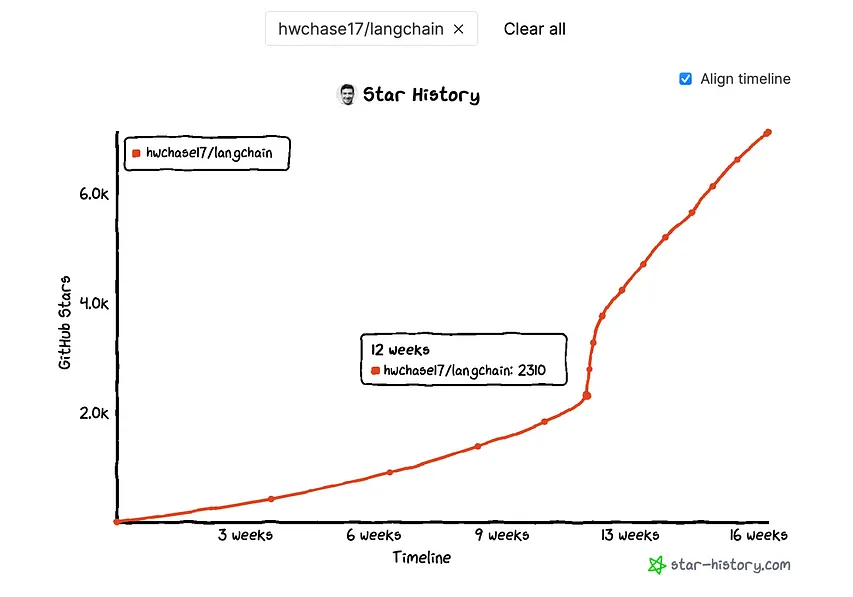
\includegraphics[width=0.6\linewidth,keepaspectratio]{langchain3}
\end{center}	  


{\tiny (Ref: Getting started with LangChain - Avra)}
\end{frame}


%%%%%%%%%%%%%%%%%%%%%%%%%%%%%%%%%%%%%%%%%%%%%%%%%%%%%%%%%%%%%%%%%%%%%%%%%%%%%%%%%%
\begin{frame}\frametitle{Why LangChain?}

\begin{itemize}
\item LLMs and Prompts: Prompt management, Prompt optimization, Generic interface for all LLMs and Common utilities for working with LLMs
\item Chains: Chains are sequences of calls that whether to an LLM or a different utility. LangChain provides a standard interface for chains, many integrations with other tools, \& end-to-end chains for common applications.
\item Extenal Data Augmentation: Specific types of chains that first interact with an external data source to fetch data to use in the generation step. Examples of this include summarization of long pieces of text \& question/answering over specific data sources
\item Agents: Agents involve an LLM making decisions about which actions to take, taking that action, seeing an observation, \& repeating that until done. LangChain provides a standard interface for agents, a selection of agents to choose from, and examples of end-to-end agents.
\item Memory: Memory refers to the concept of persisting state between calls of a chain/agent. LangChain provides a standard interface for memory, a collection of memory implementations, and examples of chains/agents that use memory.
\item Evaluation [BETA]: Generative models are notoriously hard to evaluate with traditional metrics. One new way of evaluating them is using language models themselves to do the evaluation. LangChain provides some prompts/chains for assisting in this.
\end{itemize}

{\tiny (Ref: Linkedin Post by Munjal Patel)}
\end{frame}

%%%%%%%%%%%%%%%%%%%%%%%%%%%%%%%%%%%%%%%%%%%%%%%%%%%%%%%%%%%%%%%%%%%%%%%%%%%%%%%%%%
\begin{frame}\frametitle{LangChain Usecases}

\begin{itemize}
\item Personal assistants
\item Question answering over database(s)
\item Chatbots
\item Querying tabular data
\item Interacting with APIs
\item Model Evaluation
\end{itemize}


{\tiny (Ref: Linkedin Post by Munjal Patel)}
\end{frame}


%%%%%%%%%%%%%%%%%%%%%%%%%%%%%%%%%%%%%%%%%%%%%%%%%%%%%%%%%%%%%%%%%%%%%%%%%%%%%%%%%%
\begin{frame}\frametitle{How LangChain Works?}

\begin{itemize}
\item Text is preprocessed by breaking it down into chunks or summaries, 
\item embedding them in a vector space, 
\item searching for similar chunks when a question is asked. 
\end{itemize}

\begin{center}
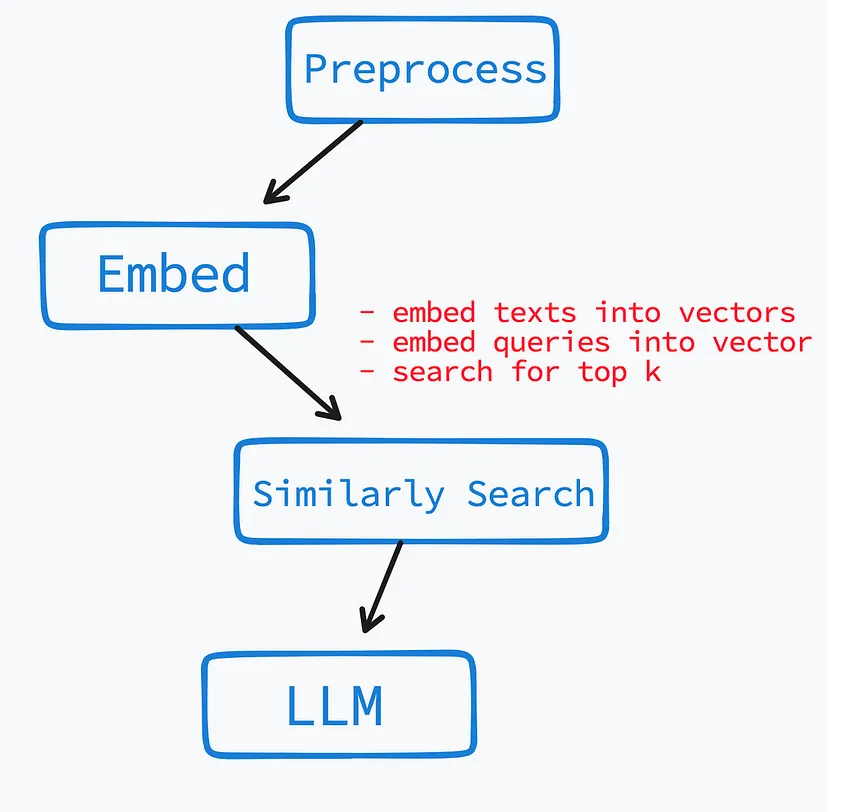
\includegraphics[width=0.5\linewidth,keepaspectratio]{langchain4}
\end{center}	  


{\tiny (Ref: Getting started with LangChain - Avra)}
\end{frame}

%%%%%%%%%%%%%%%%%%%%%%%%%%%%%%%%%%%%%%%%%%%%%%%%%%%%%%%%%%%%%%%%%%%%%%%%%%%%%%%%%%
\begin{frame}[fragile]\frametitle{LangChain Setup}

\begin{lstlisting}
pip install langchain openai cohere huggingface_hub \
ipywidgets chromadb google-search-results

import os
import langchain
from langchain.llms import OpenAI, Cohere, HuggingFaceHub
from langchain.chat_models import ChatOpenAI
from langchain.schema import (
    AIMessage,
    HumanMessage,
    SystemMessage
)
os.environ["OPENAI_API_KEY"] = ""
os.environ["COHERE_API_KEY"] = ""
os.environ["HUGGINGFACEHUB_API_TOKEN"] = ""
os.environ["SERPAPI_API_KEY"] = ""
\end{lstlisting}	  

\end{frame}

%%%%%%%%%%%%%%%%%%%%%%%%%%%%%%%%%%%%%%%%%%%%%%%%%%%%%%%%%%%%%%%%%%%%%%%%%%%%%%%%%%
\begin{frame}[fragile]\frametitle{LangChain Integrations}

\begin{lstlisting}
chatgpt = ChatOpenAI(model_name='gpt-3.5-turbo')
gpt3 = OpenAI(model_name='text-davinci-003')
cohere = Cohere(model='command-xlarge')
flan = HuggingFaceHub(repo_id="google/flan-t5-xl")

text = "How to be happy?"

print(chatgpt([HumanMessage(content=text)]))
print(gpt3(text))
print(cohere(text))
print(flan(text))
\end{lstlisting}	  

\end{frame}

%%%%%%%%%%%%%%%%%%%%%%%%%%%%%%%%%%%%%%%%%%%%%%%%%%%%%%%%%%%%%%%%%%%%%%%%%%%%%%%%%%
\begin{frame}[fragile]\frametitle{LangChain Components}

\begin{center}
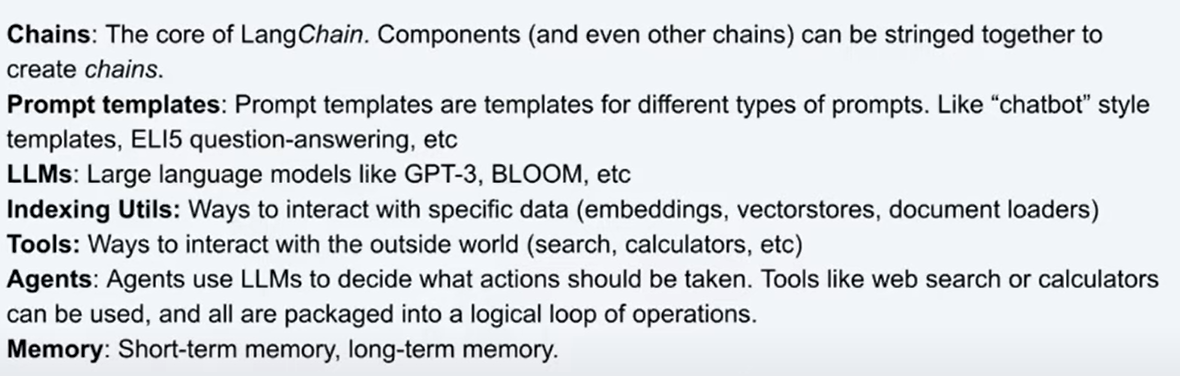
\includegraphics[width=\linewidth,keepaspectratio]{langchain1}
\end{center}	  

{\tiny (Ref: Building the Future with LLMs, LangChain, \& Pinecone)}
\end{frame}


%%%%%%%%%%%%%%%%%%%%%%%%%%%%%%%%%%%%%%%%%%%%%%%%%%%%%%%%%%%%%%%%%%%%%%%%%%%%%%%%%%
\begin{frame}[fragile]\frametitle{LangChain Data Loaders}

There are a lot of document loaders: File Loader, Directory Loader, Notion, ReadTheDocs, HTML, PDF, PowerPoint, Email, GoogleDrive, Obsidian, Roam, EverNote, YouTube, Hacker News, GitBook, S3 File, S3 Directory, GCS File, GCS Directory, Web Base, IMSDb, AZLyrics, College Confidential, Gutenberg, Airbyte Json, CoNLL-U, iFixit, Notebook, Copypaste, CSV, Facebook Chat, Image, Markdown, SRT, Telegram, URL, Word Document, Blackboard

Langchain will chunk the documents and then index its vectors.

\begin{lstlisting}
from langchain.document_loaders import TextLoader
loader = TextLoader('state_of_the_union.txt')
from langchain.indexes import VectorstoreIndexCreator
index = VectorstoreIndexCreator().from_loaders([loader])
query = "What did the president say about Ketanji Brown Jackson"
index.query(query)
\end{lstlisting}	  

\end{frame}

%%%%%%%%%%%%%%%%%%%%%%%%%%%%%%%%%%%%%%%%%%%%%%%%%%%%%%%%%%%%%%%%%%%%%%%%%%%%%%%%%%
\begin{frame}[fragile]\frametitle{LangChain Memory}

Keeps chat history in memory. You can also summarize the chat history.

\begin{lstlisting}
from langchain.llms import OpenAI
from langchain.prompts import PromptTemplate
from langchain.chains import ConversationChain
from langchain.memory import ConversationBufferWindowMemory, CombinedMemory, ConversationSummaryMemory


conv_memory = ConversationBufferWindowMemory(
    memory_key="chat_history_lines",
    input_key="input",
    k=1
)

summary_memory = ConversationSummaryMemory(llm=OpenAI(), input_key="input")
# Combined
memory = CombinedMemory(memories=[conv_memory, summary_memory])
_DEFAULT_TEMPLATE = """The following is a friendly conversation between a human and an AI. The AI is talkative and provides lots of specific details from its context. If the AI does not know the answer to a question, it truthfully says it does not know.

\end{lstlisting}	  

\end{frame}


%%%%%%%%%%%%%%%%%%%%%%%%%%%%%%%%%%%%%%%%%%%%%%%%%%%%%%%%%%%%%%%%%%%%%%%%%%%%%%%%%%
\begin{frame}[fragile]\frametitle{LangChain Memory}


\begin{lstlisting}
Summary of conversation:
{history}
Current conversation:
{chat_history_lines}
Human: {input}
AI:"""
PROMPT = PromptTemplate(
    input_variables=["history", "input", "chat_history_lines"], template=_DEFAULT_TEMPLATE
)
llm = OpenAI(temperature=0)
conversation = ConversationChain(
    llm=llm, 
    verbose=True, 
    memory=memory,
    prompt=PROMPT
)

conversation.run("Hi!")
conversation.run("Can you tell me a joke?")
conversation.run("Can you tell me a similar joke?")
\end{lstlisting}	  

\end{frame}


%%%%%%%%%%%%%%%%%%%%%%%%%%%%%%%%%%%%%%%%%%%%%%%%%%%%%%%%%%%%%%%%%%%%%%%%%%%%%%%%%%
\begin{frame}[fragile]\frametitle{Building Blocks: Inputs}

Input types that LLMs accept

\begin{itemize}
\item Simple string \lstinline|my_text = "What day comes after Friday?"|
\item For the models that handle conversations, chat message type input is needed. There are three message types to label who the sender is: system (Role), human (Prompt), and assistant (AI) for response.
\item Some LLM models accept a document as their input. A document not only includes the page content but also some meta-data such as the source and creation time.
\end{itemize}

{\tiny (Ref: Techy Stuff 3: Notes on LangChain Library - Bill)}

\begin{lstlisting}
chat = ChatOpenAI(temperature=.7, openai_api_key=openai_api_key)

chat([ SystemMessage(content="You are a nice AI bot that helps a user figure out what to eat in one short sentence"),
        HumanMessage(content="I like tomatoes, what should I eat?") ])
Document(page_content="This is my document. It is full of text that I've gathered from other places",
         metadata={'my_document_id' =234234,'my_document_source' = "The LangChain Papers",    'my_document_create_time' = 1680013019 })
\end{lstlisting}	  


\end{frame}

%%%%%%%%%%%%%%%%%%%%%%%%%%%%%%%%%%%%%%%%%%%%%%%%%%%%%%%%%%%%%%%%%%%%%%%%%%%%%%%%%%
\begin{frame}[fragile]\frametitle{Building Blocks: Models}

You provide input of a certain type (text, chat, or document) to a model, and the model will spit out a result for you.

\begin{itemize}
\item To use an LLM, you can import it from LangChain’s LLMS module.
\item The most common model is the language model that accepts a simple string input
\end{itemize}

{\tiny (Ref: Techy Stuff 3: Notes on LangChain Library - Bill)}

\begin{lstlisting}
from langchain.llms import OpenAI
llm = OpenAI(model_name="text-ada-001", openai_api_key=openai_api_key)
llm("What day comes after Friday?")
\end{lstlisting}	  


\end{frame}

%%%%%%%%%%%%%%%%%%%%%%%%%%%%%%%%%%%%%%%%%%%%%%%%%%%%%%%%%%%%%%%%%%%%%%%%%%%%%%%%%%
\begin{frame}[fragile]\frametitle{Building Blocks: Models}

 The chat model allows AI to generate a response from an array of conversations. Each conversation can be initiated by a different party such as the system, a human, and an AI assistant

{\tiny (Ref: Techy Stuff 2: Notes on Prompt Engineering - Bill)}

\begin{lstlisting}
from langchain.chat_models import ChatOpenAI
from langchain.schema import HumanMessage, SystemMessage, AIMessage

chat = ChatOpenAI(temperature=1, openai_api_key=openai_api_key)
chat(
    [
        SystemMessage(content="You are an unhelpful AI bot that makes a joke at whatever the user says"),
        HumanMessage(content="I would like to go to New York, how should I do this?")
    ]
)
\end{lstlisting}	  
\end{frame}


%%%%%%%%%%%%%%%%%%%%%%%%%%%%%%%%%%%%%%%%%%%%%%%%%%%%%%%%%%%%%%%%%%%%%%%%%%%%%%%%%%
\begin{frame}[fragile]\frametitle{Building Blocks: Models}

Text embedding model turns a string of text into a vector representation. A vector is simply an array of numbers of a set length depending on the embedding model. Each number is called a dimension.

{\tiny (Ref: Techy Stuff 2: Notes on Prompt Engineering - Bill)}

\begin{lstlisting}
from langchain.embeddings import OpenAIEmbeddings

embeddings = OpenAIEmbeddings(openai_api_key=openai_api_key)

text = "Hi! It's time for the beach"

text_embedding = embeddings.embed_query(text)
print (f"Your embedding is length {len(text_embedding)}")
print (f"Here's a sample: {text_embedding[:5]}...")

// Here's a sample: [-0.00020583387231454253, -0.003205398330464959, -0.0008301587076857686, -0.01946892775595188, -0.015162716619670391]...
\end{lstlisting}	  
\end{frame}


%%%%%%%%%%%%%%%%%%%%%%%%%%%%%%%%%%%%%%%%%%%%%%%%%%%%%%%%%%%%%%%%%%%%%%%%%%%%%%%%%%
\begin{frame}[fragile]\frametitle{Building Blocks: Prompts}

\begin{itemize}
\item You can pass a static prompt to a model and get a result, but it will be boring. 
\item For a model to provide a relevant output dynamically based on the user and the context, you need a smarter way to construct the prompt.
\item With the prompt template class, you can create a prompt that includes variables, so the content of a template can be super flexible, which can even pull data from external sources.
\end{itemize}

{\tiny (Ref: Techy Stuff 3: Notes on LangChain Library - Bill)}

\begin{lstlisting}
from langchain.llms import OpenAI
from langchain import PromptTemplate

llm = OpenAI(model_name="text-davinci-003", openai_api_key=openai_api_key)

# Notice "location" below, that is a placeholder for another value later
template = """
I really want to travel to {location}. What should I do there?

Respond in one short sentence
"""

prompt = PromptTemplate(input_variables=["location"],template=template)
final_prompt = prompt.format(location='Rome')
\end{lstlisting}	  
\end{frame}

%%%%%%%%%%%%%%%%%%%%%%%%%%%%%%%%%%%%%%%%%%%%%%%%%%%%%%%%%%%%%%%%%%%%%%%%%%%%%%%%%%
\begin{frame}[fragile]\frametitle{Building Blocks: Example Selector}

\begin{itemize}
\item One common practice to enrich a prompt is through few-shot prompting, you append a few examples before a user’s actual question/input to teach the machine how it should approach a question and format its answer.
\item If you put all the examples you have into a prompt, the length of the input might exceed the max tokens, and the API cost will be exorbitantly high.
\item Example Selector can automatically pick the relevant examples that closely relate to the user’s input and append them to a prompt for you.
\end{itemize}

{\tiny (Ref: Techy Stuff 3: Notes on LangChain Library - Bill)}

\begin{lstlisting}
from langchain.prompts import FewShotPromptTemplate, PromptTemplate
from langchain.llms import OpenAI

llm = OpenAI(model_name="text-davinci-003", openai_api_key=openai_api_key)

example_prompt = PromptTemplate(
    input_variables=["input", "output"],
    template="Example Input: {input}\nExample Output: {output}",
)

# Examples of locations that nouns are found
examples = [
    {"input": "pirate", "output": "ship"},
    {"input": "pilot", "output": "plane"},
    {"input": "driver", "output": "car"},
    {"input": "tree", "output": "ground"},
    {"input": "bird", "output": "nest"},
]
\end{lstlisting}	  
\end{frame}

%%%%%%%%%%%%%%%%%%%%%%%%%%%%%%%%%%%%%%%%%%%%%%%%%%%%%%%%%%%%%%%%%%%%%%%%%%%%%%%%%%
\begin{frame}[fragile]\frametitle{Building Blocks: Example Selector}

\begin{lstlisting}
# SemanticSimilarityExampleSelector will select examples that are similar to your input by semantic meaning

example_selector = SemanticSimilarityExampleSelector.from_examples(
    # This is the list of examples available to select from.
    examples, 
    
    # This is the embedding class used to produce embeddings which are used to measure semantic similarity.
    OpenAIEmbeddings(openai_api_key=openai_api_key), 
    
    # This is the VectorStore class that is used to store the embeddings and do a similarity search over.
    FAISS, 
    
    # This is the number of examples to produce.
    k=2
)

similar_prompt = FewShotPromptTemplate(
    # The object that will help select examples
    example_selector=example_selector,
    
    # Your prompt
    example_prompt=example_prompt,
    
    # Customizations that will be added to the top and bottom of your prompt
    prefix="Give the location an item is usually found in",
    suffix="Input: {noun}\nOutput:",
    
    # What inputs your prompt will receive
    input_variables=["noun"],
)

llm(similar_prompt.format(noun=my_noun))
\end{lstlisting}	  
\end{frame}

%%%%%%%%%%%%%%%%%%%%%%%%%%%%%%%%%%%%%%%%%%%%%%%%%%%%%%%%%%%%%%%%%%%%%%%%%%%%%%%%%%
\begin{frame}[fragile]\frametitle{Building Blocks: Indexes}

\begin{itemize}
\item What should you do if you want to ask GPT to summarize a 300-page novel for you? 
\item GPT has set a max token on the user’s input so you cannot just copy and paste the whole document into a prompt. 
\item For a model to consume a longer text, we have to use a technique called indexes, and here are the steps we have to perform:
\begin{itemize}
\item Load the document (think of it as a 300-page novel in PDF format)
\item Split the text into chunks (set the max tokens for each chunk)
\item Embed the chunks into vectors with the embedding model
\item Store them in a vector database
\item Retrieve the relevant chunks when building a prompt dynamically
\end{itemize}
\end{itemize}

{\tiny (Ref: Techy Stuff 3: Notes on LangChain Library - Bill)}

\end{frame}

%%%%%%%%%%%%%%%%%%%%%%%%%%%%%%%%%%%%%%%%%%%%%%%%%%%%%%%%%%%%%%%%%%%%%%%%%%%%%%%%%%
\begin{frame}[fragile]\frametitle{Building Blocks: Indexes}

Here is the example code:


\begin{lstlisting}
from langchain.document_loaders import TextLoader
from langchain.text_splitter import RecursiveCharacterTextSplitter
from langchain.vectorstores import FAISS
from langchain.embeddings import OpenAIEmbeddings

loader = TextLoader('data/PaulGrahamEssays/worked.txt')
documents = loader.load()

# Get your splitter ready
text_splitter = RecursiveCharacterTextSplitter(chunk_size=1000, chunk_overlap=50)

# Split your docs into texts
texts = text_splitter.split_documents(documents)

# Get embedding engine ready
embeddings = OpenAIEmbeddings(openai_api_key=openai_api_key)

# Embedd your texts
db = FAISS.from_documents(texts, embeddings)

# Init your retriever. Asking for just 1 document back
retriever = db.as_retriever()

docs = retriever.get_relevant_documents("what types of things did the author want to build?")
\end{lstlisting}	  
\end{frame}


%%%%%%%%%%%%%%%%%%%%%%%%%%%%%%%%%%%%%%%%%%%%%%%%%%%%%%%%%%%%%%%%%%%%%%%%%%%%%%%%%%
\begin{frame}\frametitle{Chains}

\begin{itemize}
\item Enable users to combine multiple components together to create a single, coherent application.
\item Example: takes user input, formats it using a PromptTemplate, and then passes the formatted response to a Large Language Model (LLM) for processing.
\item Sequential chains: output of the first LLM becomes the input to the second LLM and so on
\end{itemize}

\begin{center}
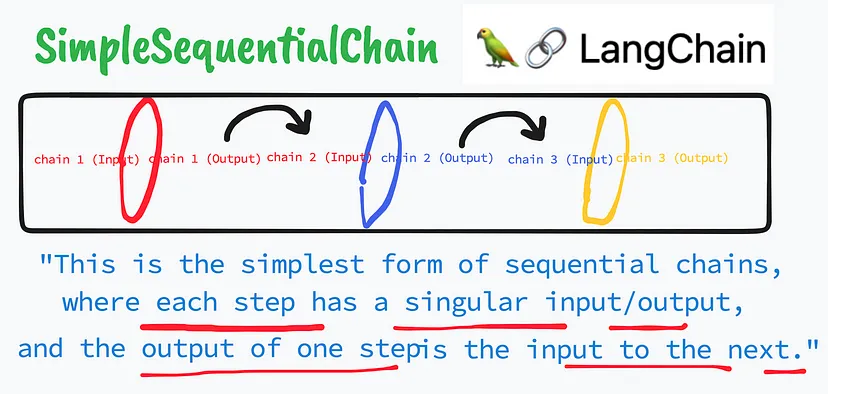
\includegraphics[width=0.8\linewidth,keepaspectratio]{langchain5}
\end{center}	  


{\tiny (Ref: Getting started with LangChain - Avra)}
\end{frame}

%%%%%%%%%%%%%%%%%%%%%%%%%%%%%%%%%%%%%%%%%%%%%%%%%%%%%%%%%%%%%%%%%%%%%%%%%%%%%%%%%%
\begin{frame}[fragile]\frametitle{LangChain Chain}


\begin{lstlisting}
from langchain.chat_models import ChatOpenAI
from langchain import LLMChain
from langchain.prompts.chat import (
    ChatPromptTemplate,
    HumanMessagePromptTemplate,
)
human_message_prompt = HumanMessagePromptTemplate(
        prompt=PromptTemplate(
            template="What is a good name for a company that makes {product}?",
            input_variables=["product"],
        )
    )
chat_prompt_template = ChatPromptTemplate.from_messages([human_message_prompt])
chat = ChatOpenAI(temperature=0.9)
chain = LLMChain(llm=chat, prompt=chat_prompt_template)
print(chain.run("colorful socks"))

\end{lstlisting}	  

\end{frame}


%%%%%%%%%%%%%%%%%%%%%%%%%%%%%%%%%%%%%%%%%%%%%%%%%%%%%%%%%%%%%%%%%%%%%%%%%%%%%%%%%%
\begin{frame}[fragile]\frametitle{LangChain Chain}


\begin{lstlisting}

second_prompt = PromptTemplate(
    input_variables=["company_name"],
    template="Write a catchphrase for the following company: {company_name}",
)
chain_two = LLMChain(llm=llm, prompt=second_prompt)

from langchain.chains import SimpleSequentialChain
overall_chain = SimpleSequentialChain(chains=[chain, chain_two], verbose=True)

# Run the chain specifying only the input variable for the first chain.
catchphrase = overall_chain.run("colorful socks")
print(catchphrase)
\end{lstlisting}	  

\end{frame}

%%%%%%%%%%%%%%%%%%%%%%%%%%%%%%%%%%%%%%%%%%%%%%%%%%%%%%%%%%%%%%%%%%%%%%%%%%%%%%%%%%
\begin{frame}[fragile]\frametitle{LangChain Agent}

Use various LLMs with external tools, like 'serpapi' to do Google search.

First search api finds who the girlfreind is, then it uses calculator to do the maths.

\begin{lstlisting}
from langchain.agents import load_tools
from langchain.agents import initialize_agent

tools = load_tools(["serpapi", "llm-math"], llm=gpt3)
agent = initialize_agent(tools, llm=gpt3, agent="zero-shot-react-description", verbose=True)
agent.run("Who is Leo DiCaprio's girlfriend? What is her current age raised to the 0.43 power?")
\end{lstlisting}	  

\end{frame}

%%%%%%%%%%%%%%%%%%%%%%%%%%%%%%%%%%%%%%%%%%%%%%%%%%%%%%%%%%%%%%%%%%%%%%%%%%%%%%%%%%
\begin{frame}[fragile]\frametitle{Chains, another example}

{\tiny (Ref: Getting started with LangChain - Avra)}


\begin{lstlisting}
    # Chain 1: Generating a rephrased version of the user's question
    template = """{question}\n\n"""
    prompt_template = PromptTemplate(input_variables=["question"], template=template)
    question_chain = LLMChain(llm=llm, prompt=prompt_template)

    # Chain 2: Generating assumptions made in the statement
    template = """Here is a statement:
        {statement}
        Make a bullet point list of the assumptions you made when producing the above statement.\n\n"""
    prompt_template = PromptTemplate(input_variables=["statement"], template=template)
    assumptions_chain = LLMChain(llm=llm, prompt=prompt_template)
    assumptions_chain_seq = SimpleSequentialChain(
        chains=[question_chain, assumptions_chain], verbose=True
    )

\end{lstlisting}

\end{frame}

%%%%%%%%%%%%%%%%%%%%%%%%%%%%%%%%%%%%%%%%%%%%%%%%%%%%%%%%%%%%%%%%%%%%%%%%%%%%%%%%%%
\begin{frame}[fragile]\frametitle{Chains}

{\tiny (Ref: Getting started with LangChain - Avra)}


\begin{lstlisting}
    # Chain 3: Fact checking the assumptions
    template = """Here is a bullet point list of assertions:
    {assertions}
    For each assertion, determine whether it is true or false. If it is false, explain why.\n\n"""
    prompt_template = PromptTemplate(input_variables=["assertions"], template=template)
    fact_checker_chain = LLMChain(llm=llm, prompt=prompt_template)
    fact_checker_chain_seq = SimpleSequentialChain(
        chains=[question_chain, assumptions_chain, fact_checker_chain], verbose=True)
    # Final Chain: Generating the final answer to the user's question based on the facts and assumptions
    template = """In light of the above facts, how would you answer the question '{}'""".format(user_question)
    template = """{facts}\n""" + template
    prompt_template = PromptTemplate(input_variables=["facts"], template=template)
    answer_chain = LLMChain(llm=llm, prompt=prompt_template)
    overall_chain = SimpleSequentialChain(
        chains=[question_chain, assumptions_chain, fact_checker_chain, answer_chain],
        verbose=True,)
\end{lstlisting}


\end{frame}

%%%%%%%%%%%%%%%%%%%%%%%%%%%%%%%%%%%%%%%%%%%%%%%%%%%%%%%%%%%%%%%%%%%%%%%%%%%%%%%%%%
\begin{frame}\frametitle{Chains}

The SimpleSequentialChain combines several chains of operations to run a pipeline. 

\begin{itemize}
\item question\_chain: This chain takes the user's question as input and returns it as output. 
\item assumptions\_chain: This chain takes the output from question\_chain as input and produces a bullet-point list of assumptions based on a statement related to the question. 
\item fact\_checker\_chain: This chain takes the outputs from question\_chain and assumptions\_chain as inputs and produces a bullet-point list of assertions based on the question and assumptions.
\item answer\_chain: This chain takes the outputs from question\_chain, assumptions\_chain, and fact\_checker\_chain as inputs and produces an answer to the user's question based on the facts generated by the previous chains.
\end{itemize}


{\tiny (Ref: Getting started with LangChain - Avra)}
\end{frame}


%%%%%%%%%%%%%%%%%%%%%%%%%%%%%%%%%%%%%%%%%%%%%%%%%%%%%%%%%%%%%%%%%%%%%%%%%%%%%%%%%%
\begin{frame}\frametitle{Prompt Engineering}

\begin{center}
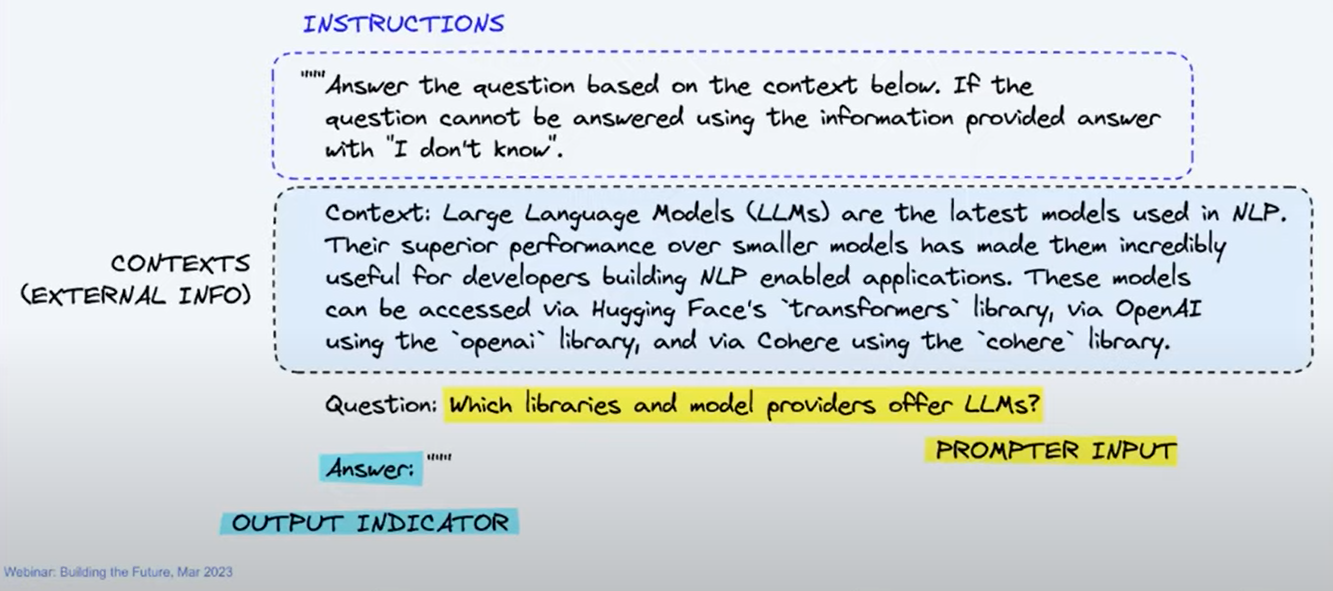
\includegraphics[width=\linewidth,keepaspectratio]{langchain2}
\end{center}	  

{\tiny (Ref: Building the Future with LLMs, LangChain, \& Pinecone)}
\end{frame}

%%%%%%%%%%%%%%%%%%%%%%%%%%%%%%%%%%%%%%%%%%%%%%%%%%%%%%%%%%%%%%%%%%%%%%%%%%%%%%%%%%
\begin{frame}\frametitle{References}


\begin{itemize}
\item Official doc: https://docs.langchain.com/docs/
\item Git Repo: https://github.com/hwchase17/langchain
\item Cookbook by Gregory Kamradt(Easy way to get started): https://github.com/gkamradt/langchain-tutorials/blob/main/LangChain\%20Cookbook.ipynb
\item Youtube Tutorials: https://www.youtube.com/watch?v=\_v\_fgW2SkkQ\&list=PLqZXAkvF1bPNQER9mLmDbntNfSpzdDIU5
\end{itemize}


\end{frame}